\documentclass[a4paper,10pt]{article}
\usepackage[utf8]{inputenc}
\usepackage[T1]{fontenc}
\usepackage{lmodern}
\usepackage[margin=1.4cm, top=1.2cm, bottom=1.2cm]{geometry}
\usepackage{hyperref}
\usepackage{xcolor}
\usepackage{enumitem}
\usepackage{graphicx}
\usepackage{titlesec}

% Minimal clean styling
\hypersetup{colorlinks=true, urlcolor=blue!70!black, linkcolor=blue!70!black}
\pagestyle{empty}
\setlength{\parindent}{0pt}

% Section formatting
\titleformat{\section}{\large\bfseries\color{black}}{}{0em}{}[\titlerule]
\titlespacing*{\section}{0pt}{6pt}{4pt}

% Colors
\definecolor{accent}{RGB}{20, 50, 120}

% Role command
\newcommand{\role}[4]{%
 \vspace{2pt}\noindent
 \begin{minipage}[t]{0.70\textwidth}\raggedright\textbf{#1} \textbullet\ \textit{#3}\end{minipage}%
 \hfill
 \begin{minipage}[t]{0.28\textwidth}\raggedleft\footnotesize\color{gray}#2 \textbullet\ #4\end{minipage}%
 \vspace{1pt}%
}
\setlist[itemize]{leftmargin=1.2em, itemsep=1.5pt, topsep=2pt, parsep=0pt}

\begin{document}

% ================= HEADER (HEADLINE is tailored) =================
\begin{minipage}[c]{0.80\textwidth}
 {\Huge\bfseries Prabhavit Gupta}\\[3pt]
 {\color{accent}\large AI Engineer: Agent Architecture, MCP Orchestration \& Next.js Full-Stack}\\[6pt]
 {\footnotesize +39 351 610 7807 ~$\vert$~
 \href{mailto:prabhavitg@gmail.com}{prabhavitg@gmail.com} ~$\vert$~
 \href{https://www.linkedin.com/in/prabhavit/}{linkedin.com/in/prabhavit} ~$\vert$~
 \href{https://github.com/prab-gupta}{github.com/prab-gupta} ~$\vert$~
 Venice, Italy}
\end{minipage}\hfill
\begin{minipage}[c]{0.18\textwidth}
 \raggedleft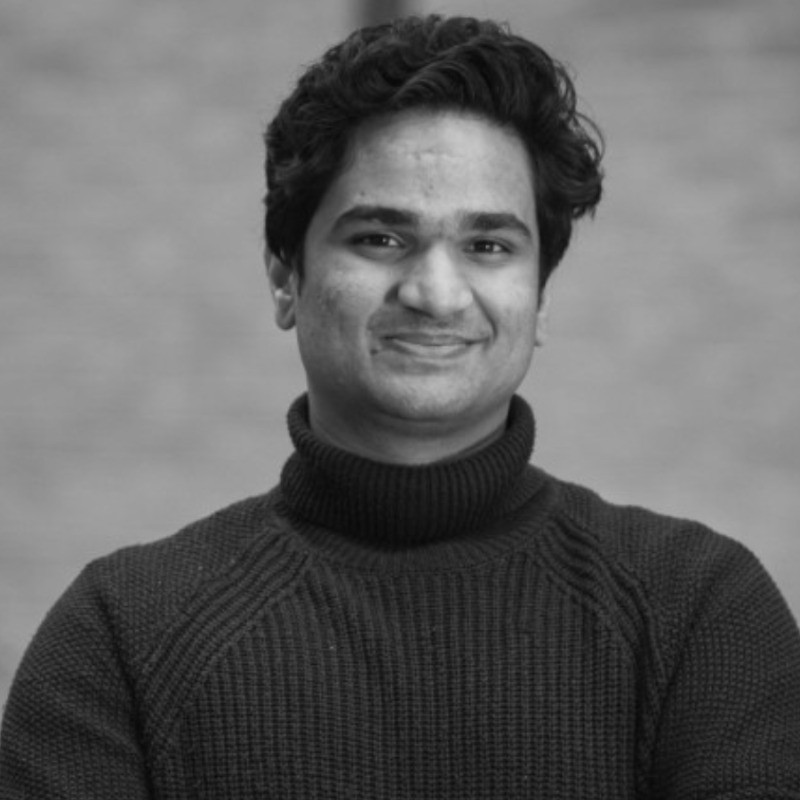
\includegraphics[width=2.0cm]{photo.jpg}
\end{minipage}
\vspace{-2pt}

% ================= SUMMARY (tailored) =================
\section{Summary}
AI and software engineer with hands-on experience building production agent workflows, Model Context Protocol (MCP) integrations, and full-stack web applications. At FlowSpace, engineered autonomous document processing agents, integrated customer support AI operating against live backend data, and led migration off a legacy stack to a modern Next.js product with background jobs and REST APIs. Experienced implementing tool-calling, structured LLM outputs, WebSockets, and Supabase/PostgreSQL backends. Based in the EU with unrestricted European work authorization; available immediately.

% ================= EXPERIENCE (frozen) =================
\section{Experience}

\role{\href{https://flowspace.co}{FlowSpace.co}}{Mar 2024 - Aug 2026}{Lead Developer (Full-time, Freelance)}{London, UK (remote)}
\begin{itemize}
 \item Built an AI listing bot with a human in the loop: it takes a brochure in any format (PDF, web page, photo or spreadsheet), drafts the full listing with an LLM, and pushes it to the backend after review. 900+ listings drafted.
 \item Streamlined customer support with AI agents that answer queries against live platform data and escalate to a person on low confidence.
 \item Integrated the OfficeRnD and Nexudus APIs for automated bookings, and built CRM lead-capture integration and GTM automations (sales funnel, lead enrichment, outbound) with n8n.
 \item Led the migration off a legacy stack to a coded Next.js and Laravel product: mapped the data model, chose the migration path per entity (API or CSV) and drove the cutover. Scaled the platform from 2,000 to 4,500+ users.
 \item Documented product and business logic with the developer team, coordinated between the internal team and an external agency, and built a commute-time calculator tool for companies.
 \item \textit{Tools: Claude Code, n8n, Playwright, Postman, Laravel, TypeScript, Supabase, GitHub, Jira, ClickUp, Miro, Google Analytics, Microsoft Clarity}
\end{itemize}

\role{Urlink}{Apr 2025 - Jul 2025}{Project Manager \& AI-Assisted Developer (Freelance)}{Barcelona, Spain}
\begin{itemize}
 \item Built automated workflows and structured customer-facing demos with AI agents for client onboarding and document ingestion.
 \item Managed project delivery end to end: mapped stakeholder requirements, built proof-of-concept prototypes, coordinated testing, and handed over documentation to client teams.
 \item \textit{Tools: Claude Code, Python, APIs, Postman, Supabase}
\end{itemize}

\role{Freelance}{Sep 2023 - Mar 2024}{Full-Stack AI \& Automation Developer}{Venice, Italy}
\begin{itemize}
 \item Built web scrapers, data enrichment pipelines, and custom API integrations for clients across Europe.
 \item Developed internal tools with modern frontend frameworks and backend scripts, automating repetitive manual data entry.
 \item \textit{Tools: TypeScript, Python, n8n, Supabase, REST APIs}
\end{itemize}

\role{\href{https://tractionboard.co}{Tractionboard.co}}{Aug 2023 - Oct 2023}{Low-Code Developer (Internship)}{Utrecht, Netherlands}
\begin{itemize}
 \item Integrated ChatGPT/OpenAI and Sendgrid, built responsive designs, debugged features and implemented Google Ads 4.
 \item \textit{Tools: Figma, Sendgrid, ChatGPT}
\end{itemize}

% ================= EDUCATION (frozen) =================
\section{Education}
\role{Ca' Foscari University of Venice}{Oct 2020 - Jun 2024}{Bachelor's in Philosophy, International Studies \& Economics, Minor in Entrepreneurship}{Venice, Italy}

% ================= CERTIFICATIONS (frozen) =================
\section{Certifications}
Microsoft Copilot Studio Agent Academy \textbullet\ Microsoft: Introduction to building AI agents \textbullet\ Microsoft Power Automate \textbullet\ Tray.AI Build Practitioner (Sep 2024) \textbullet\ Tray.AI Build Foundations

% ================= ADDITIONAL INFORMATION (frozen) =================
\section{Additional Information}
\begin{itemize}
 \item \textbf{Work authorization:} European Long Term Residence Permit (Italy), no sponsorship needed in the EU. Available immediately.
 \item \textbf{Languages:} Hindi (native), English (professional), Italian (beginner).
\end{itemize}

% ================= CORE SKILLS (tailored, at the bottom) =================
\section{Core Skills}
\begin{itemize}
 \item \textbf{AI Agents \& Orchestration:} Open-source agent architectures, Model Context Protocol (MCP), tool-use, memory management, structured outputs, prompt engineering, Claude and OpenAI APIs
 \item \textbf{Full-Stack Engineering:} Next.js, React, TypeScript, Python (working level), WebSockets, REST APIs, auth, background jobs, Laravel
 \item \textbf{Data \& Infrastructure:} PostgreSQL, Supabase, Redis, Docker, Git/GitHub, Playwright automated testing, API monitoring
 \item \textbf{Production Delivery:} System architecture, rapid prototyping, cross-functional collaboration, async delivery across Europe
\end{itemize}

\end{document}
